\RequirePackage[orthodox]{nag}
\documentclass[11pt]{article}

%% Define the include path
\makeatletter
\providecommand*{\input@path}{}
\g@addto@macro\input@path{{include/}{../include/}}
\makeatother

\usepackage{../../include/akazachk}


\title{ECH4905 ChemE Optimization HW 4}
\author{Andres Espinosa}

\begin{document}
\maketitle

\section{Problem 1}
Consider the nonlinear program
\begin{align*}
  \text{minimize} & \quad x_1^2 + 2x_2^2 \\
  \text{subject to} & \quad x_1^2 + x_2^2 \leq 5 \\
  & \quad 2x_1 - 2x_2 = 1
\end{align*}

\subsection{Part a}
Write the KKT conditions for the problem
\label{p1:kkt}

\textbf{Solution: }
The KKT conditions must satisfy stationarity, complementary slackness, primal feasibility, and dual feasibility.
In order to find these conditions, we calculate the following gradients for the stationarity condition
\begin{align*}
  \nabla f_0(\textbf{x}) =
  \begin{bmatrix}
    2x_1 \\ 4x_2
  \end{bmatrix}
  , \quad
  \nabla f_1(\textbf{x}) = 
  \begin{bmatrix}
    2x_1 \\ 2x_2
  \end{bmatrix}
  , \quad
  \nabla g(\textbf{x}) = 
  \begin{bmatrix}
    2 \\ -2
  \end{bmatrix}
\end{align*}

The KKT conditions are then

\begin{align*}
  \begin{bmatrix}
    2x_1 \\ 4x_2
  \end{bmatrix}
  +
  \lambda
  \begin{bmatrix}
    2x_1 \\ 2x_2
  \end{bmatrix}
  +
  \nu
  \begin{bmatrix}
    2 \\ -2
  \end{bmatrix}
  = \textbf{0}
  & \quad \text{Stationarity} \\
  \lambda (x_1^2 + x_2^2 - 5) = 0 
  & \quad \text{Complementary Slackness} \\
  x_1^2 + x_2^2 - 5 \leq 0, \quad 2x_1 - 2x_2 - 1 = 0
  & \quad \text{Primal Feasibility} \\
  \lambda \geq 0 
  & \quad \text{Dual Feasibility}
\end{align*}

\subsection{Part b}
Using \ref{p1:kkt} and other conditions for optimality, what can you conclude about the following solutions to the nonlinear program
\begin{align*}
  \textbf{x} = 
  \begin{bmatrix}
    0 \\ 0
  \end{bmatrix}
  , \quad
  \textbf{x} = 
  \begin{bmatrix}
    1 \\ \frac{1}{2}
  \end{bmatrix}
  , \quad 
  \textbf{x} = 
  \begin{bmatrix}
    \frac{1}{3} \\ -\frac{1}{6}
  \end{bmatrix}
\end{align*}

\textbf{Solution: }
For the first point, $\textbf{x} = [0,0]$, the primal feasibility is violated because $2(0) - 2(0) -1 \neq 0$.
Therefore, this point is not feasible in the original problem and therefore not optimal.

For the second point, $\textbf{x} = [1, \frac{1}{2}]$, the following are the KKT conditions
\begin{align*}
  \begin{bmatrix}
    2 \\ 2
  \end{bmatrix}
  +
  \lambda
  \begin{bmatrix}
    2 \\ 1
  \end{bmatrix}
  +
  \nu
  \begin{bmatrix}
    2 \\ -2
  \end{bmatrix}
  = \textbf{0}
  & \quad \text{Stationarity} \\
  \lambda (1 + \frac{1}{4} - 5) = 0 
  & \quad \text{Complementary Slackness} \\
  1 + \frac{1}{4} - 5 \leq 0, \quad 2 - 1 - 1 = 0
  & \quad \text{Primal Feasibility} \\
  \lambda \geq 0 
  & \quad \text{Dual Feasibility}
\end{align*}
Since $\lambda=0$ due to the complementary slackness condition, the stationary condition is not satisfied.

For the third point, $\textbf{x} = [\frac{1}{3}, -\frac{1}{6}]$, the following are the KKT conditions
\begin{align*}
  \begin{bmatrix}
    \frac{2}{3} \\ -\frac{2}{3}
  \end{bmatrix}
  +
  \lambda
  \begin{bmatrix}
    \frac{2}{3} \\ -\frac{1}{3}
  \end{bmatrix}
  +
  \nu
  \begin{bmatrix}
    2 \\ -2
  \end{bmatrix}
  = \textbf{0}
  & \quad \text{Stationarity} \\
  \lambda (\frac{1}{9} + \frac{1}{36} - 5) = 0 
  & \quad \text{Complementary Slackness} \\
  \frac{1}{9} + \frac{1}{36} - 5 \leq 0, \quad \frac{2}{3} + \frac{1}{3} - 1 = 0
  & \quad \text{Primal Feasibility} \\
  \lambda \geq 0 
  & \quad \text{Dual Feasibility}
\end{align*}
These conditions are satisfied with $\lambda=0, \nu=-\frac{1}{3}$.
Therefore, this point $[\frac{1}{3}, -\frac{1}{6}]$ is an optimal point to the convex optimization problem above.


\section{Problem 2}
Consider the following flowsheet:

\begin{figure}[htbp]
  \centerline{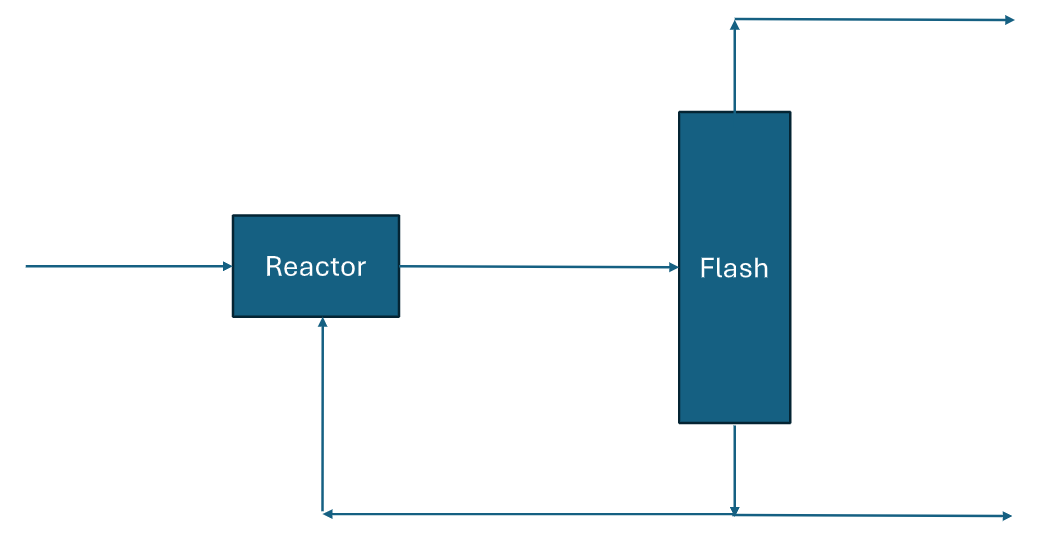
\includegraphics[width=0.5\textwidth]{images/flowsheet.png}}
  \label{fig:flowsheet}
\end{figure}

Assume that the following reaction takes place with a 50\% conversion. The feed to
the reactor consists of pure A.
\[ A \rightarrow B \]
The flash separator can be modeled as a perfect separation unit, capable of
producing any required purity.
We assume that the purge fraction should be between 1\% to 99\%.
The profit is given by the following equation:
\[ 0.5B_{\text{Top}} - 0.1F_R(500 - T) - 10^{-5}V \]
Where $B_{\text{Top}}$ is the molar flow B exiting as top product from the flash separator. 
And $F_R$ is the recycle molar flow rate.

\subsection{Part a}
Formulate a model of this process.




\textbf{Solution: }
We define the following variables
\begin{itemize}
  \item $F_{A0}$: The input flow of A from the left of the reactor.
  \item $F_{AF}$: The output flow of A from the bottom of the flash 
  \item $F_{AR}$: The input flow of A from the recycle stream of the splitter.
  \item $F_{AP}$: The output flow of A that is purged to the right of the splitter.
  \item $F_{AI}$: The intermediate flow of A from the reactor to the flash.
  \item $F_{BI}$: The intermediate flow of B from the reactor to the flash.
  \item $F_{BTop}$: The output flow of B from the top of the flash.
  \item $\lambda$: The split fraction of the splitter.
  \item $T$: Temperature
  \item $V$: Pressure (set to the input flow)
\end{itemize}

We then have the following optimization problem

\begin{align*}
  \text{maximize} & \quad 0.5 F_{BTop} - 0.1F_{AR}(500-T) - 10^{-5} V & \text{Objective}\\
  \text{subject to} & \quad F_{A0} + F_{AR} = F_{AI} + F_{BI} & \text{Reactor MB}\\
  & \quad F_{AI} + F_{BI} = F_{BTop} + F_{AF} & \text{Flash MB} \\
  & \quad F_{AI} = F_{BI} & \text{Reactor Conversion}\\
  & \quad F_{BTop} = F_{BI} & \text{Separate flow B}\\
  & \quad F_{AI} = F_{AF} & \text{Separate flow A} \\
  & \quad F_{AF} = F_{AR} + F_{AP} & \text{Splitter MB} \\
  & \quad F_{AR} = \lambda F_{AF} & \text{Recycle Split} \\
  & \quad F_{AP} = (1-\lambda) F_{AF} & \text{Purge Split} \\
  & \quad \textbf{F} \succeq 0 & \text{Non-Negativity} \\
  & \quad 0 \leq \lambda \leq 1 & \text{Split Proportion} \\
  & \quad 273 \leq T \leq 500 & \text{Temperature Constraints} \\
  & \quad V = F_{A0} & \text{Pressure Constraint} \\
  & \quad 0.01(F_{AP} + F_{AR}) \leq F_{AP} \leq 0.99(F_{AP} + F_{AR}) & \text{Purge Fraction}
\end{align*}
Note that since the split is only two ways, only one variable is used and that avoids an otherwise additional constraint of $\textbf{1}^\top \lambda = 1$

\subsection{Part b}
Set up the model in GAMS and try 3 different NLP solvers, compare the results.

\textbf{Solution: }
The following code was used to solve the problem. 
The three solvers used, \texttt{baron, gurobi, conopt} resulted in the same answers.
Currently, an arbitrary input bound of 1000 is used so that the solver doesnt push the value of the input flow to infinity.
I didn't see anything in the problem that naturally constrained the input flow, so I picked a value of 1000.

\begin{verbatim}
Variables
    profit profit equation;

Positive Variables
    FA0 reactor input of A
    FAF flash output of A
    FAR splitter recycle output of A
    FAP splitter purge output of A
    FAI reactor output of A
    FBI reactor output of B
    FBTop flash output of B
    V pressure
    T temperature
    lambda split fraction;
    
    
Equations
    profit_e
    reactor_mb
    flash_mb
    reactor_cons
    sep_B
    sep_A
    split_mb
    recycle_split
    purge_split
    split_prop_l
    temp_l
    temp_g
    pressure
    purge_frac_l
    purge_frac_g
    arbitrary_input_bound;
profit_e.. profit =e= 0.5 * FBTop - 0.1* FAR * (500-T) - 0.00001 * V;

reactor_mb.. FA0 + FAR =e= FAI + FBI;
flash_mb.. FAI + FBI =e= FBTop + FAF;
reactor_cons.. FAI =e= FBI;
sep_B.. FBTop =e= FBI;
sep_A.. FAI =e= FAF;
split_mb.. FAF =e= FAR + FAP;
recycle_split.. FAR =e= lambda * FAF; 
purge_split.. FAP =e= (1-lambda) * FAF;
split_prop_l.. lambda =l= 1;
temp_l.. T =l= 500;
temp_g.. T =g= 273;
pressure.. V =e= FA0;
purge_frac_l.. 0.01* (FAP + FAR) =l= FAP;
purge_frac_g.. FAP =l= 0.99*(FAP + FAR);
arbitrary_input_bound.. FA0 =l= 1000; 

Model flowsheet /all/ ;

*option nlp=gurobi;
*option nlp=conopt;
option nlp=baron;

Solve flowsheet using nlp maximizing profit;

Solution      = 495.039504950495  best solution found during preprocessing
Best possible = 495.039504950495
Absolute gap  = 5.6843418860808E-14  optca = 1E-9
Relative gap  = 1.14826025584549E-16  optcr = 0.0001


                           LOWER          LEVEL          UPPER

---- EQU profit_e            .       9.095765E-15          .          
---- EQU reactor_mb          .       -2.27374E-13          .          
---- EQU flash_mb            .              .              .          
---- EQU reactor_c~          .              .              .          
---- EQU sep_B               .              .              .          
---- EQU sep_A               .              .              .          
---- EQU split_mb            .       4.618528E-14          .          
---- EQU recycle_s~          .       1.197122E-10          .          
---- EQU purge_spl~          .       -1.19703E-10          .          
---- EQU split_pro~        -INF            0.9900         1.0000      
---- EQU temp_l            -INF          500.0000       500.0000      
---- EQU temp_g           273.0000       500.0000        +INF         
---- EQU pressure            .              .              .          
---- EQU purge_fra~        -INF      -1.23110E-14          .          
---- EQU purge_fra~        -INF         -970.2970          .          
---- EQU arbitrary~        -INF         1000.0000      1000.0000      

                           LOWER          LEVEL          UPPER

---- VAR profit            -INF          495.0395        +INF         
---- VAR FA0                 .          1000.0000        +INF         
---- VAR FAF                 .           990.0990        +INF         
---- VAR FAR                 .           980.1980        +INF         
---- VAR FAP                 .             9.9010        +INF         
---- VAR FAI                 .           990.0990        +INF         
---- VAR FBI                 .           990.0990        +INF         
---- VAR FBTop               .           990.0990        +INF         
---- VAR V                   .          1000.0000        +INF         
---- VAR T                   .           500.0000        +INF         
---- VAR lambda              .             0.9900        +INF         

\end{verbatim}



\end{document}